\documentclass[11pt]{article}

% Use final mode for the public arXiv version.
\usepackage[final]{acl}

% Standard package includes
\usepackage{times}
\usepackage{latexsym}
\usepackage[T1]{fontenc}
\usepackage[utf8]{inputenc}
\usepackage{microtype}
\setlength{\emergencystretch}{2em}
\usepackage{inconsolata}
\usepackage{graphicx}
\usepackage{booktabs}
\usepackage{multirow}
\usepackage{tabularx}
\usepackage{fvextra}
\usepackage{amssymb}
\DefineVerbatimEnvironment{SPARQL}{Verbatim}{breaklines=true,breakanywhere=true,fontsize=\small}

\title{PIPE-RDF: Execution-Grounded Generation of Schema-Specific NL--SPARQL Benchmarks}

\author{
  Suraj Ranganath \\
  UC San Diego \\
  \texttt{suranganath@ucsd.edu}
}

\begin{document}
\maketitle

\begin{abstract}
Natural-language access to RDF knowledge graphs depends on evaluation sets whose queries actually run on the graph being tested. Existing KGQA benchmarks provide useful shared tasks, but their schemas, namespaces, predicates, and query distributions often differ from the graphs used in practice. We introduce PIPE-RDF, an execution-grounded workflow for building schema-specific natural-language/SPARQL benchmarks from a target RDF graph. PIPE-RDF starts with reverse queries that populate deterministic binding banks, uses category-aware retrieval to supply schema-matched examples, and applies controlled LLM generation to produce candidate question-query pairs. Each candidate is accepted only after passing predicate and type checks, deduplication, parsing, execution, answer-shape validation, and non-empty-result checks. Across a compact company-location schema and a 25M-triple LDBC Semantic Publishing Benchmark graph, PIPE-RDF produces 3{,}600 balanced pairs across nine query categories with no parse, execution, or empty-answer failures in the released artifacts. Cross-model probes, a dual LLM-judge audit, and downstream prompting experiments indicate that the resulting benchmarks are robust, semantically aligned, and useful as schema-matched examples for NL--SPARQL evaluation.
\end{abstract}

\section{Introduction}
RDF knowledge graphs expose structured data through SPARQL, but natural-language access to those graphs remains highly schema-dependent. A natural-language question can be fluent while its corresponding query uses the wrong predicate, assumes a missing type, or returns an answer set that cannot exist in the target graph. This makes benchmark construction a first-order problem for NL--SPARQL work: an evaluation set must reflect the target ontology, prefixes, available attributes, and intended query categories before it can be used to compare parsers or retrieval strategies.

Public KGQA benchmarks such as LC-QuAD, QALD-9-plus, and Mintaka provide valuable shared test beds, but they are tied to fixed public schemas and entity distributions \citep{Trivedi_2017,perevalov2022qald9plusmultilingualdatasetquestion,sen2022mintakacomplexnaturalmultilingual}. They do not directly answer a common methodological question: given a new RDF schema, how can we construct a balanced, executable, and auditable NL--SPARQL benchmark without manually authoring every query? Modern large language models (LLMs) can help generate candidate questions and queries \citep{brown2020languagemodelsfewshotlearners,touvron2023llamaopenefficientfoundation}, but unconstrained generation is prone to unsupported entities, invalid predicates, and semantically plausible but unanswerable queries.

PIPE-RDF addresses this benchmark-construction problem with a pipeline that grounds generation in graph facts. The central mechanism is reverse querying: before a question--query pair is accepted, the system first finds entity bindings that satisfy the intended template in the target graph. Category-balanced generation, retrieval-augmented prompting, predicate/type whitelists, deduplication, execution validation, and repair are then used to produce benchmark artifacts that are not merely grammatical, but executable against a fixed RDF endpoint.

\textbf{Contributions.} We:
\begin{itemize}
  \item propose a three-phase pipeline for schema-specific NL--SPARQL benchmark generation with reverse-query grounding and execution validation;
  \item evaluate PIPE-RDF on a fixed company-location schema and a large LDBC Semantic Publishing Benchmark (SPB) graph with a broader schema profile, producing 3{,}600 accepted Phase-3 pairs across nine categories;
  \item report operational metrics including parse validity, execution success, empty-result rates, repair rates, materialized generation attempts, endpoint latency, and predicate usage;
  \item add cross-model robustness probes and a compact downstream utility evaluation for zero-shot versus retrieval-augmented NL-to-SPARQL prompting;
  \item report a dual LLM-judge semantic audit with agreement, Cohen's \(\kappa\), consensus error categories, and the exact judging prompt.
\end{itemize}

\section{Background and Related Work}
\textbf{Benchmark coverage and query taxonomies.} NL--SPARQL and KGQA benchmarks have been developed through several complementary traditions. LC-QuAD, LC-QuAD 2.0, QALD-9-plus, and Spider4SPARQL provide question--query pairs over public graphs and established ontologies \citep{Trivedi_2017,DBLP:conf/semweb/DubeyBA019,perevalov2022qald9plusmultilingualdatasetquestion,DBLP:conf/bigdataconf/KostenCS23}. CFQ uses SPARQL over Freebase-style data to stress compositional generalization \citep{keysers2020cfq}, and KQA Pro provides explicit compositional programs plus SPARQL for complex KBQA \citep{cao-etal-2022-kqa}. Mintaka explicitly balances query categories (counting, comparative, superlative, ordinal, multi-hop, intersection, difference/negation, yes/no, and generic) to avoid skewed evaluation \citep{sen2022mintakacomplexnaturalmultilingual}. These datasets are valuable shared test beds, but their schemas and entity distributions are fixed once released. PIPE-RDF instead targets the complementary problem of constructing an executable benchmark for a user-specified RDF schema.

\textbf{Template and workload generation.} Earlier SPARQL dataset and workload generators show that template instantiation and workload design are central for RDF evaluation. Neural SPARQL Machines generate synthetic NL--SPARQL training pairs from templates over DBpedia-style data \citep{soru2017sparqlforeignlanguage}. RDF engine benchmarks such as SP2Bench, LDBC SPB, and FEASIBLE study scalable SPARQL workload generation and query-log or feature-driven benchmark construction \citep{schmidt2009sp2bench,ldbcspb,DBLP:conf/semweb/SaleemMN15}. PIPE-RDF builds on this lineage but adds LLM-era NL generation, category-specific retrieval, binding-bank construction, and strict accepted-record validation for schema-specific KGQA artifacts rather than triplestore throughput alone.

\textbf{Retrieval augmentation and prompting.} Retrieval-augmented generation (RAG) improves text-to-query performance by conditioning on relevant examples and schema cues \citep{lewis2021retrievalaugmentedgenerationknowledgeintensivenlp}. In practice, RAG offers a low-cost alternative to fine-tuning when schema-specific examples are scarce. PIPE-RDF maintains category-specific retrieval banks to provide structurally similar NL--SPARQL pairs during generation, reducing cross-category drift and improving template grounding.

\textbf{Validity and evaluation.} Grammar-constrained decoding (e.g., PICARD) improves syntactic correctness for structured query generation \citep{Scholak_2021}. SPARQL-specific constrained decoding such as SPARKLE integrates KG structure during inference to reduce inexecutable query generation \citep{lee2025sparkle}. SPARQL-specific metrics such as SP-BLEU/SP-F1 normalize variables for fairer matching \citep{Rony_2022}, while code-oriented structural metrics such as CodeBLEU inspire future extensions \citep{ren2020codebleumethodautomaticevaluation}. LLM-as-judge protocols such as G-Eval and MT-Bench show that strong model judges can provide scalable rubric-based judgments when prompts and outputs are logged \citep{liu-etal-2023-g,zheng2023mtbench}. PIPE-RDF combines execution, parsing, structural, and dual-judge semantic metrics so that accepted artifacts can be audited beyond surface validity.

\textbf{Agentic and verification-heavy NL--SPARQL systems.} Recent systems such as GRASP, FIRESPARQL, and Chatty-KG use LLM agents, decomposition, verification, or conversational orchestration to answer questions over knowledge graphs \citep{walter2025grasp,pan2025firesparql,omar2025chattykg}. PIPE-RDF is complementary: it does not propose a new inference-time question-answering agent, but constructs schema-specific, executable benchmark artifacts that can evaluate or supply retrieval/fine-tuning examples for such systems.

\textbf{Synthetic text-to-query benchmarks.} Synthetic benchmark construction is also active outside RDF. For example, SM3-Text-to-Query builds a synthetic multi-model medical text-to-query benchmark across heterogeneous data models \citep{furst2024sm3}. PIPE-RDF makes a different trade-off: it targets RDF/SPARQL specifically and prioritizes graph-grounded executability, schema whitelists, category balance, and released audit logs over unconstrained linguistic breadth.

\textbf{LLM-driven workload generation for analytics.} Recent work on cross-model analytics workload generation uses a two-stage design (reverse query generation followed by NL query generation), explicit schema/strategy controls, and detailed error analyses across model families \citep{zheng2024crossmodel}. We adopt the same design principle of schema-grounded workload construction, and the released artifacts log strategy tags and failure modes to make benchmark generation auditable beyond aggregate success rates.

\textbf{Comparison with existing approaches.} Table~\ref{tab:comparison} contrasts PIPE-RDF with prominent KGQA and SPARQL workload-generation methodologies. Our novelty is not a new semantic parser or the isolated use of templates. The contribution is an integrated, reproducible construction pipeline that combines graph-grounded binding banks, category-aware LLM prompting, strict acceptance filters, LLM semantic judging, and run-level observability for new RDF schemas.

\begin{table}[t]
  \centering
  \small
  \resizebox{\linewidth}{!}{
	  \begin{tabular}{lcccc}
	    \toprule
	    Feature & Public KGQA & CFQ/KQA & RDF workloads & \textbf{PIPE-RDF} \\
	    \midrule
	    Released NL--SPARQL pairs & \(\checkmark\) & \(\checkmark\) & -- & \(\checkmark\) \\
	    New-schema configuration & -- & --/partial & \(\checkmark\) & \(\checkmark\) \\
	    Graph-grounded bindings & partial & partial & \(\checkmark\) & \(\checkmark\) \\
	    Category-balanced generation & partial & \(\checkmark\) & -- & \(\checkmark\) \\
	    LLM generation/RAG controls & -- & -- & -- & \(\checkmark\) \\
	    Execution + semantic audit & partial & partial & \(\checkmark\) & \(\checkmark\) \\
	    \bottomrule
	  \end{tabular}
	  }
	  \caption{Comparison of PIPE-RDF with existing KGQA datasets and RDF workload-generation approaches. PIPE-RDF targets schema-specific NL--SPARQL benchmark construction with both graph-grounded generation and accepted-record auditing. ``Partial'' denotes support that is limited to fixed released benchmarks or does not directly handle user-provided schemas.}
  \label{tab:comparison}
\end{table}

\section{Benchmark Design Goals}
PIPE-RDF is designed to meet four goals for schema-specific benchmark construction: (i) \textbf{schema fidelity} - generated queries must be grounded in a fixed schema and valid predicates; (ii) \textbf{category balance} - benchmarks should cover complex query types rather than skew toward easy factoids; (iii) \textbf{operational observability} - generation, parsing, and execution outcomes must be logged for debugging and cost control; and (iv) \textbf{maintainability} - the pipeline should be repeatable as schemas evolve, minimizing manual curation. These goals shape the pipeline phases, validation logic, and artifact outputs.

\section{Category Taxonomy}
To prevent evaluation bias, PIPE-RDF follows a nine-category taxonomy derived from complex KGQA datasets \citep{sen2022mintakacomplexnaturalmultilingual}. Each category maps to distinct SPARQL constructs (e.g., aggregations, ordering, multi-hop joins) and therefore stresses different failure modes. Table~\ref{tab:categories} summarizes the taxonomy and example question patterns used in Schema C.

\begin{table}[t]
  \centering
  \scriptsize
  \setlength{\tabcolsep}{3pt}
  \begin{tabular}{>{\raggedright\arraybackslash}p{0.17\linewidth} >{\raggedright\arraybackslash}p{0.16\linewidth} >{\raggedright\arraybackslash}p{0.57\linewidth}}
    \toprule
    Category & SPARQL construct & Example pattern \\
    \midrule
    Generic & single triple & Who is a key person at {company}? \\
    Counting & COUNT & How many companies are in {location}? \\
    Comparative & boolean comparison & Do {company1} and {company2} differ in size? \\
    Superlative & ordering & Which company has most employees? \\
    Ordinal & ranked ordering & Which company was founded second earliest? \\
    Multi-hop & join chains & Which location has companies with key persons? \\
    Intersection & conjunction & Which companies are in {location} and {industry}? \\
    Difference & boolean exclusion & Are {company1} and {company2} in different industries? \\
    Yes/No & boolean check & Is {company} located in {location}? \\
    \bottomrule
  \end{tabular}
  \caption{Category taxonomy used for balanced benchmark generation.}
  \label{tab:categories}
\end{table}

\section{PIPE-RDF Methodology}
PIPE-RDF is a three-phase pipeline (Figure~\ref{fig:pipeline}) designed to generate schema-specific benchmarks while minimizing unanswerable or out-of-schema queries.

\textbf{Phase 1: seed generation.} The pipeline prompts an LLM to produce NL templates from a schema summary. We represent each template as a tuple \((c, q_{\theta}, s, r_{\theta}, v_c)\), where \(c\) is the category, \(q_{\theta}\) is an NL pattern with typed slots, \(s\) is the slot-type map, \(r_{\theta}\) is a reverse SPARQL pattern that returns candidate bindings for the slots, and \(v_c\) is the category validator. Each template is validated by \emph{reverse querying}: the system generates or renders a SPARQL query that searches the KG for entity bindings satisfying the template. Valid bindings instantiate the template and the resulting NL--SPARQL pairs are stored as seeds for later retrieval.

\textbf{Phase 2: category-wise seeding.} Templates are generated per category and paired with retrieval-augmented prompts using Phase-1 seeds. Outputs are validated by execution, optionally repaired, and stored in category-specific retrieval banks. This step ensures early coverage of complex query structures (e.g., aggregations, comparisons, multi-hop joins) and prevents domination by simple templates.

\textbf{Phase 3: full dataset generation.} The pipeline generates batches per category using category-specific retrieval banks. Each candidate is parsed, executed, and logged. Records are retained only after strict acceptance checks, then exported as balanced CSV/JSONL artifacts with run summaries.

\textbf{Prompt construction and retrieval.} Prompts combine (i) a task description, (ii) the schema summary, (iii) a small set of retrieved NL--SPARQL examples, and (iv) the target question. Retrieval is category-aware, which narrows the space of candidate structures and reduces cross-category drift. The ARR runs use top-$k=3$ to balance example coverage against prompt length.

\textbf{Reverse querying and schema control.} Reverse queries build deterministic binding banks for each template before generation. Each bank stores a bounded pool of valid entity/literal bindings, and Phase 3 samples from those banks client-side rather than repeatedly issuing randomized SPARQL queries. This avoids broad \texttt{ORDER BY RAND()} scans on large repositories and makes GraphDB work an explicit upfront stage. We also batch label and type resolution for candidate URIs with \texttt{VALUES} clauses, reducing thousands of small endpoint calls. We enforce explicit predicate/type whitelists and slot-type hints (company, location, person, industry) to ensure every generated query conforms to the target schema. Duplicate questions are filtered using token-level Jaccard similarity (threshold 0.97 in the ARR runs), and a stall limit prevents repeated template regeneration when no new valid rows are found.

\textbf{Validation and repair.} Each generated SPARQL query is parsed and executed; failures trigger a repair prompt that attempts to correct syntax and predicate usage. Repairs are logged and included in run summaries for operational tracking. The expanded runs use a stricter acceptance gate than the original baseline: accepted records must parse, execute, return a non-empty answer object, and match the expected answer type for the category. Boolean \texttt{ASK} queries therefore produce explicit true/false answers rather than empty-result negatives. The primary benchmark is an answerable evaluation split, so zero-count counting questions are excluded from this split rather than mixed with positive counting examples; controlled zero-count diagnostics can be generated as a separate negative split using the same template interface. Post-generation, category-specific pattern enforcement can normalize output forms (e.g., \texttt{ASK} for boolean checks, \texttt{DISTINCT} for set-returning categories, \texttt{COUNT(DISTINCT ...)} for counting queries, and deterministic \texttt{LIMIT~1} tie-breaking for superlative/ordinal queries). We also run a deterministic same/different lexical-shape check for comparative and difference questions, preventing records whose question asks for sameness while the query tests inequality, or vice versa. While PIPE-RDF does not require constrained decoding, it can integrate grammar-based constraints (e.g., PICARD) or KG-aware decoding (e.g., SPARKLE) to improve parse validity at inference time \citep{Scholak_2021,lee2025sparkle}.

\textbf{Curation controls.} The pipeline supports optional curation after each phase, with the ability to discard, edit, or inject examples. This is useful for sparse relations, sensitive attributes, or domain-specific naming conventions where automated validation alone may not capture all semantic constraints.

\begin{figure}[t]
  \centering
  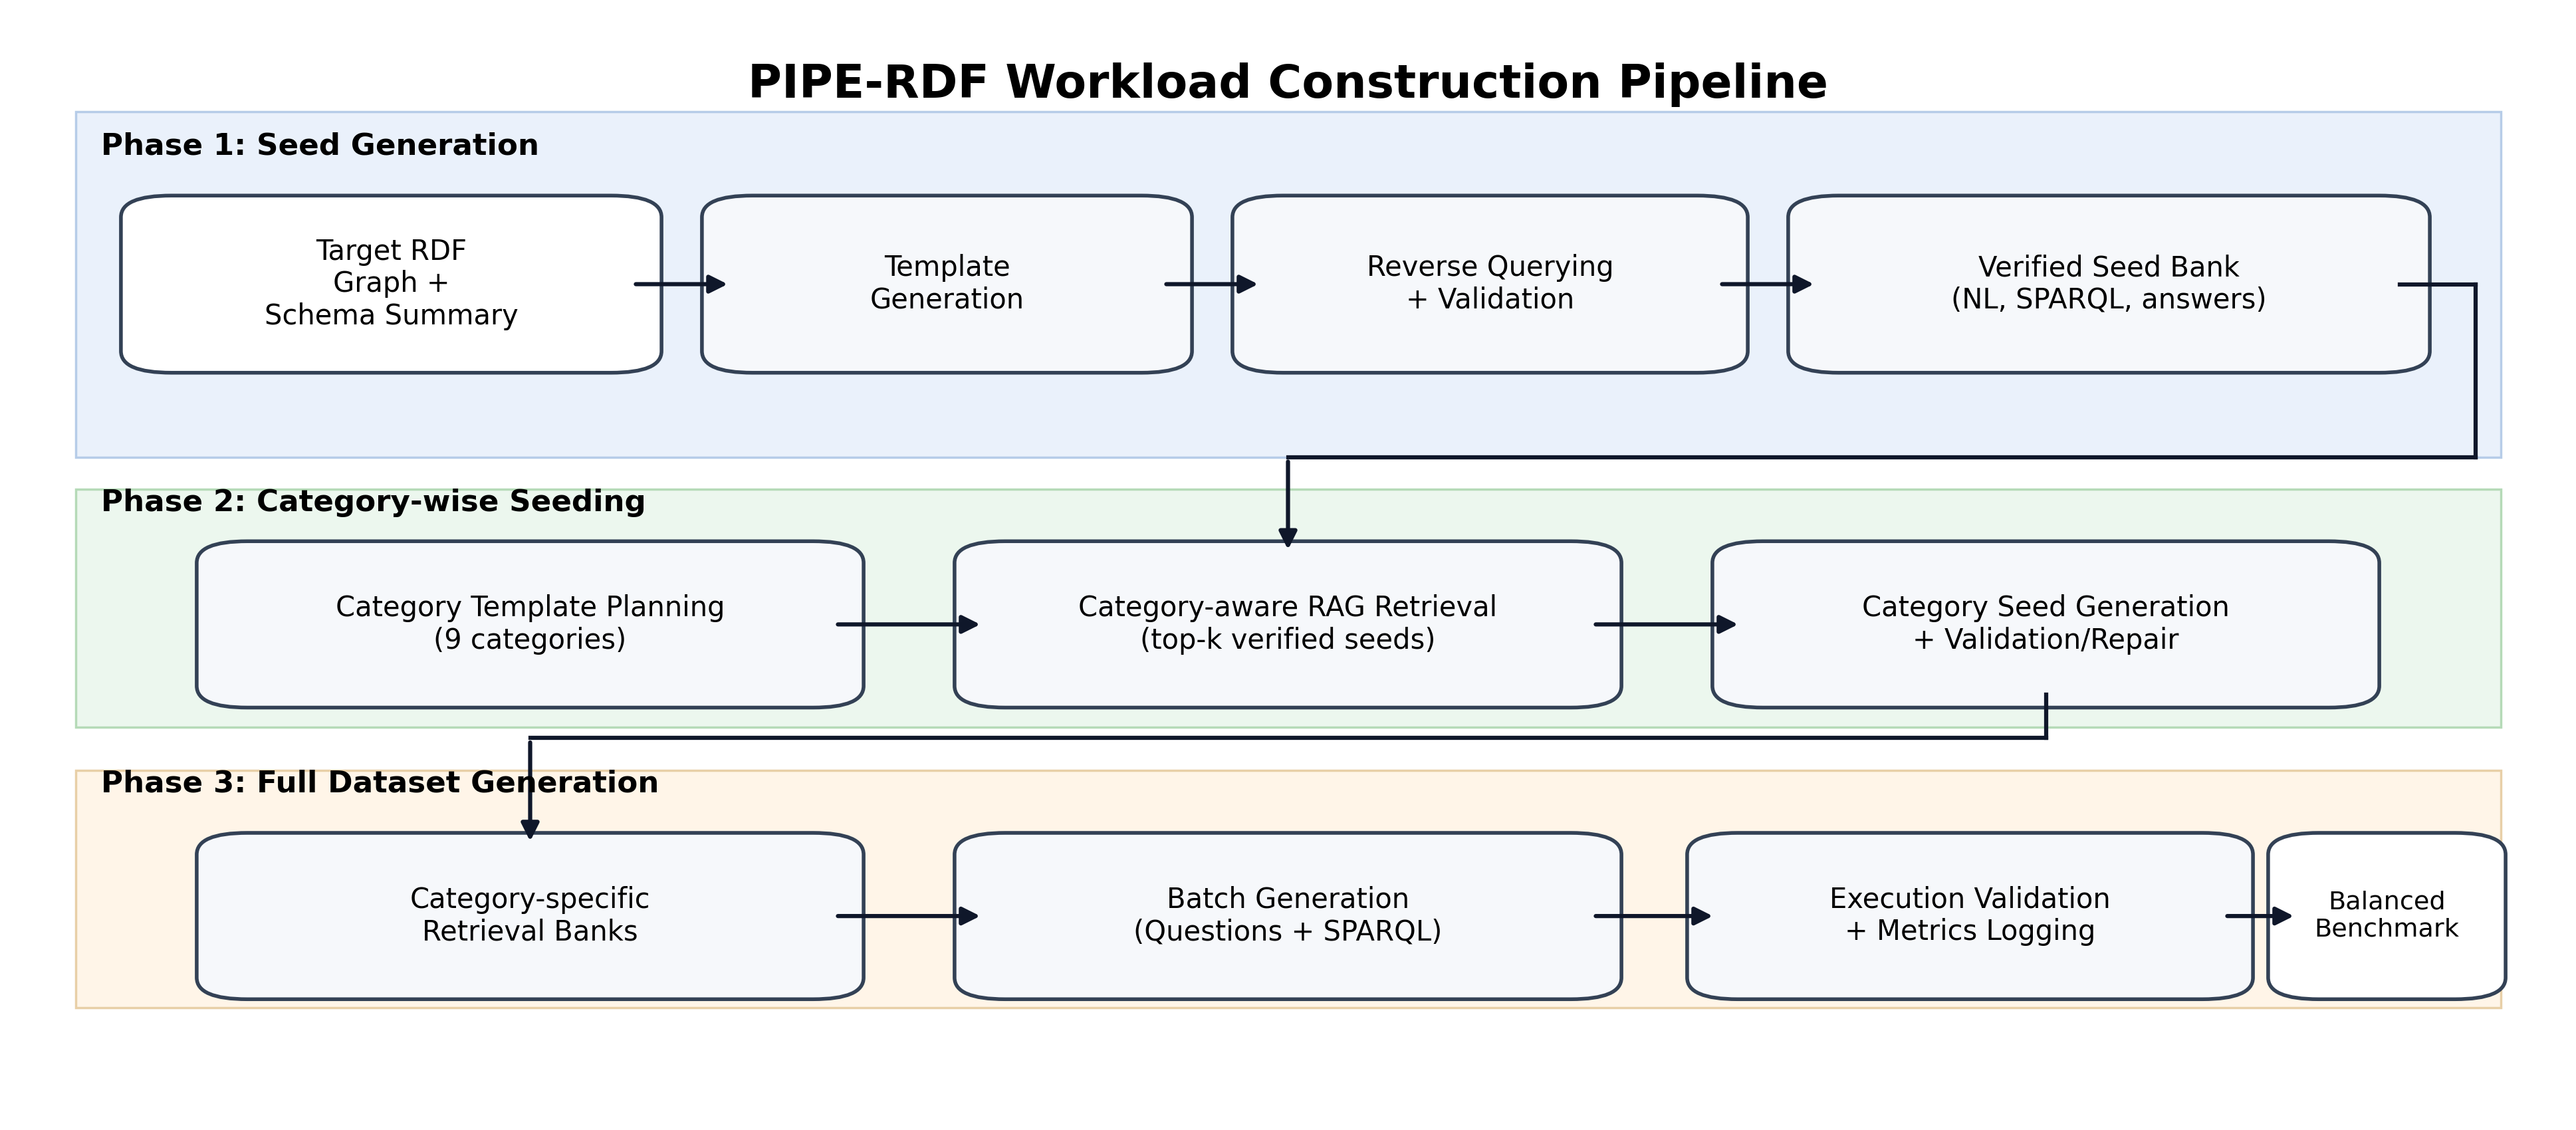
\includegraphics[width=0.95\linewidth]{figures/pipeline_architecture.png}
  \caption{PIPE-RDF workload-construction pipeline: Phase 1 uses reverse query generation to build verified seeds; Phase 2 constructs category-specific seed banks; Phase 3 generates the balanced benchmark with execution-driven validation/repair.}
  \label{fig:pipeline}
\end{figure}

\section{Schemas and Implementation}
\textbf{Fixed schema slice.} We derive a company-location mini-slice (Schema C) with 5{,}000 companies, three explicit classes (\texttt{dbo:Company}, \texttt{gn:Feature} for locations, and \texttt{foaf:Person} for key people), and industry IRIs used as labeled attribute values rather than an explicit typed class. The allowed predicates are \texttt{dbo:location}, \texttt{dbo:industry}, \texttt{dbo:keyPerson}, \texttt{dbo:foundingYear}, \texttt{dbo:numberOfEmployees}, and label predicates (\texttt{rdfs:label}, \texttt{spb:prefLabel}, \texttt{foaf:name}). This fixed schema avoids prompt drift and simplifies validation.

\textbf{Slice extraction.} The mini-slice is sampled from a public RDF source by selecting companies with at least one of the core predicates (location, industry, key person, founding year, or employee count). Linked entities (locations and key people) are included with minimal labels to support question instantiation without introducing extraneous schema elements. We intentionally exclude unrelated predicates to reduce template drift and ensure that reverse querying remains tractable.

\textbf{SPB-full schema.} To test the same method beyond the compact slice, we also run on a full LDBC Semantic Publishing Benchmark graph with roughly 25M triples. The graph has a much broader profile than Schema C (5{,}695 distinct predicates and 19{,}033 distinct types in the profiler output); its top predicates include \texttt{rdf:type}, \texttt{spb:prefLabel}, \texttt{foaf:name}, \texttt{dbo:birthPlace}, \texttt{dbo:location}, \texttt{dbo:foundingYear}, \texttt{dbo:industry}, \texttt{dbo:keyPerson}, and \texttt{dbo:numberOfEmployees}. For comparability, the benchmark-generation task still targets the company/location/person-style query categories, while the schema summary and whitelist are derived from the larger graph. This tests graph scale and broader schema-profile handling while holding the task taxonomy fixed; it is not intended as exhaustive coverage of every predicate or advanced SPARQL construct in SPB.

\textbf{Schema profiling and curation effort.} Schema profiles are produced automatically from the endpoint: \texttt{scripts/profile\_schema.py} exports predicate counts, type counts, a class--predicate matrix, and a compact schema summary. The remaining schema-specific input is a YAML configuration containing preferred types, slot-type hints, endpoint settings, and whitelist controls. In the ARR runs, Schema C explicitly lists 9 allowed predicates and 3 allowed types; SPB-full uses profiler-derived predicate/type CSVs with top-\(k\) limits plus 5 slot-type hints. The hand-authored schema-specific portion is therefore inspectable in the released YAMLs: types, slot hints, and whitelist settings, while predicate/type counts and summaries are generated by the profiler. This keeps portability work localized to the config and profiler outputs rather than hard-coding schema logic in the generator.

\begin{table}[t]
  \centering
  \small
  \setlength{\tabcolsep}{4pt}
  \begin{tabularx}{\linewidth}{>{\raggedright\arraybackslash}p{0.26\linewidth} X}
    \toprule
    Class & Key predicates/attributes \\
    \midrule
    \texttt{dbo:Company} & \texttt{dbo:location}, \texttt{dbo:industry}, \texttt{dbo:keyPerson}, \\
    & \texttt{dbo:foundingYear}, \texttt{dbo:numberOfEmployees}, \texttt{rdfs:label} \\
    \texttt{gn:Feature} & \texttt{rdfs:label}, \texttt{spb:prefLabel} \\
    \texttt{foaf:Person} & \texttt{foaf:name}, \texttt{rdfs:label} \\
    \bottomrule
  \end{tabularx}
	  \caption{Schema C mini-slice explicit classes and allowed predicates. Industry is represented as an IRI-valued company attribute and may not have an explicit \texttt{rdf:type}.}
  \label{tab:schema}
\end{table}

\textbf{Pipeline configuration.} The primary ARR runs use 8 Phase-1 templates per category, 10 Phase-1 seed instantiations per template, 50 Phase-2 seeds per category, and 200 accepted Phase-3 targets per category on each schema (3{,}600 accepted Phase-3 pairs total). Generated SPARQL is capped at 5 results to limit execution cost. Binding banks use bounded deterministic pools and client-side shuffling for diversity.

\begin{table}[t]
  \centering
  \small
  \resizebox{\linewidth}{!}{
  \begin{tabular}{ll}
    \toprule
    Parameter & Value \\
    \midrule
	    Phase 1 templates / category & 8 \\
	    Phase 1 seeds / template & 10 \\
	    Phase 2 seeds / category & 50 \\
	    Phase 3 accepted targets / category & 200 primary / 50 probe \\
	    Binding-bank target rows & 500 (Schema C) / 1{,}500 (SPB-full) \\
	    Retrieval top-$k$ & 3 \\
	    SPARQL result cap & 5 \\
	    Dedup Jaccard threshold & 0.97 \\
    \bottomrule
  \end{tabular}
  }
\caption{Key primary-run configuration. The expanded runs keep the same category taxonomy while scaling accepted Phase-3 targets and moving reverse-query work into deterministic binding-bank construction.}
  \label{tab:config}
\end{table}

\textbf{Runtime environment.} We run GraphDB 10.6.3 and execute SPARQL with inference disabled. The expanded generation uses Qwen 3.5 models served through vLLM and local \texttt{BAAI/bge-m3} embeddings. The primary runs use \texttt{Qwen/Qwen3.5-4B}; robustness probes use \texttt{Qwen/Qwen3.5-2B}, \texttt{Qwen/Qwen3.5-4B}, and \texttt{Qwen/Qwen3.5-9B}. All runs are logged with execution latency, parse validity, and answer counts; artifacts are exported as JSONL/CSV and summarized in run-level reports. A compact reproducibility checklist is provided in Appendix Section~\ref{app:repro}.

\textbf{SPARQL formalism and schema constraints.} To ensure semantic correctness, we enforce canonical query patterns:
\begin{itemize}
  \item \textbf{Counting}: Use \texttt{COUNT(DISTINCT ?var)} to avoid overcounting due to multiple bindings.
  \item \textbf{Superlative/Ordinal}: Include deterministic tie-breaking via \texttt{ORDER BY ... ?entity} to ensure reproducible results.
  \item \textbf{Numeric comparisons}: Cast literals to \texttt{xsd:integer} where applicable (e.g., \texttt{dbo:numberOfEmployees}).
  \item \textbf{Yes/No}: Use \texttt{ASK \{\}} for explicit boolean returns, avoiding empty-result ambiguity.
\end{itemize}
Schema constraints are enforced via predicate whitelists: \texttt{dbo:location} ranges over \texttt{gn:Feature}, \texttt{dbo:keyPerson} ranges over \texttt{foaf:Person}, and \texttt{dbo:foundingYear}/\texttt{dbo:numberOfEmployees} are typed literals. Label resolution prioritizes \texttt{foaf:name} for persons, \texttt{rdfs:label} for companies, and \texttt{spb:prefLabel} for locations.

\section{Evaluation Protocol}
PIPE-RDF logs operational and structural metrics for generated and accepted records. We track: (i) parse validity and execution success, (ii) non-empty answer coverage, (iii) repair attempts, (iv) materialized generation attempts and failures from run logs, (v) answer counts, (vi) prompt and question lengths, (vii) model and endpoint latency when generated by the active run, and (viii) SPARQL structural complexity (triple pattern counts, FILTER clauses, aggregations). We also compute natural-language surface diagnostics over accepted artifacts: unique-question rate, mean question length, and Distinct-1/Distinct-2. These metrics support both data quality analysis and model evaluation. While PIPE-RDF focuses on execution-driven correctness, the artifacts can be augmented with SPARQL-specific metrics (SP-F1) and structural metrics (CodeBLEU) for model evaluation \citep{Rony_2022,ren2020codebleumethodautomaticevaluation}. We also record retrieval scores to analyze the relationship between example similarity and downstream execution success.

Following recent workload-generation evaluation practice \citep{zheng2024crossmodel}, the released logs also include strategy tags inferred from query operators (JOIN, FILTER, COUNT, ORDER, NEGATION, ASK, RAG-context). These diagnostics are intended for run auditing and failure analysis rather than as the central acceptance criterion.

\textbf{Semantic correctness audit.} To measure whether generated NL--SPARQL pairs are semantically aligned (not just syntactically valid), we construct a 216-pair stratified audit packet: 2 schemas \(\times\) 9 categories \(\times\) 12 pairs. We run two independent LLM judges, GPT-5-mini and Grok-4.20-0309 non-reasoning, with the same rubric and temperature 0. Each judge checks whether (i) question intent matches the SPARQL semantics, (ii) entity bindings in the question correspond to VALUES clauses or equivalent query constraints, (iii) the answer type matches the expected return, and (iv) the category label matches the dominant SPARQL construct. We report per-judge pass rates, inter-judge agreement, Cohen's \(\kappa\), consensus pass rate, and consensus error categories. The audit packet, raw per-judge outputs, adjudicated CSV/JSONL files, and prompt are released with the artifact bundle; the exact prompt is included in Appendix Section~\ref{app:llm_judge_prompt}.

\section{Benchmark Results}
The primary expanded evaluation uses \texttt{Qwen/Qwen3.5-4B} served through vLLM. We retain 1{,}800 accepted Phase-3 pairs for each schema, with exactly 200 pairs in each of the nine categories. Table~\ref{tab:arr_schema_scale} summarizes the strict final-artifact checks. A record is accepted only if its SPARQL parses, executes, returns a category-appropriate answer object, avoids zero-count counting artifacts, and passes category-form checks such as \texttt{COUNT} for counting and ranked \texttt{ORDER BY}/\texttt{OFFSET} forms for ordinal queries. These are selection-conditioned checks on the released artifacts, not a claim that every intermediate LLM proposal is correct. Both schemas satisfy the final checks without repair calls in the released accepted artifacts. The non-empty gate does not remove boolean negatives: the accepted \texttt{ASK} categories include 28 false answers for Schema C and 224 false answers for SPB-full.

\begin{table}[t]
  \centering
  \small
  \resizebox{\linewidth}{!}{
  \begin{tabular}{lrrrrrr}
    \toprule
    Schema & Pairs & Cat. & Parse fail & Exec fail & Empty & Repairs \\
    \midrule
    Schema C & 1{,}800 & 200/200 & 0 & 0 & 0 & 0 \\
    SPB-full & 1{,}800 & 200/200 & 0 & 0 & 0 & 0 \\
    \bottomrule
  \end{tabular}
  }
  \caption{Primary expanded Phase-3 results. Both schemas are balanced at 200 examples per category across nine categories and pass strict parse, execution, answer-type, and category-form checks.}
  \label{tab:arr_schema_scale}
\end{table}

\begin{table}[t]
  \centering
  \scriptsize
  \resizebox{\linewidth}{!}{
  \begin{tabular}{lrrrrrrr}
    \toprule
    Schema & Runs & Wall h & P3 attempts & Final & Yield\% & Repairs (P3) & SPARQL ms \\
    \midrule
    Schema C & 3 & 8.01 & 2{,}692 & 1{,}800 & 66.9 & 32 (1) & 4.0 \\
    SPB-full & 2 & 3.73 & 1{,}947 & 1{,}800 & 92.4 & 23 (0) & 7.2 \\
    \bottomrule
  \end{tabular}
  }
  \caption{Operational efficiency from the contributing primary and top-up run logs. Phase-3 attempts count materialized candidates that reached validation logging; final counts the released exactly balanced artifact; yield is final retained records divided by Phase-3 attempts. Valid Phase-3 records emitted before final category replacement/deduplication were 2{,}686 for Schema C and 1{,}946 for SPB-full. Repairs are all-phase counts with Phase-3 counts in parentheses.}
  \label{tab:primary_runtime}
\end{table}

\paragraph{Question diversity and structural profile.}
Table~\ref{tab:linguistic_structural} summarizes automatic diagnostics for the two strict accepted artifacts. Each schema has 100\% unique surface questions within the released 1{,}800-pair artifact. Distinct-1/2 are surface-form diagnostics rather than human naturalness scores, and should be interpreted alongside the fixed schema and category taxonomy. The SPARQL profile reflects the target taxonomy: \texttt{ASK} appears in boolean categories, \texttt{COUNT} in counting and some boolean cardinality comparisons, and \texttt{ORDER BY} in ranked categories. SPB-full also includes limited \texttt{OPTIONAL} usage in accepted comparative/difference records, while the current taxonomy does not target property paths, named graphs, or broad \texttt{UNION} coverage.

\begin{table}[t]
  \centering
  \scriptsize
  \resizebox{\linewidth}{!}{
  \begin{tabular}{lrrrrrrrrrr}
    \toprule
    Schema & Unique Q\% & Tok. & Dist-1 & Dist-2 & Triples & FILTER\% & COUNT\% & ORDER\% & ASK\% & OPT\% \\
    \midrule
    Schema C & 100.0 & 9.8 & 9.8 & 20.3 & 2.9 & 22.7 & 11.6 & 22.2 & 33.3 & 0.0 \\
    SPB-full & 100.0 & 10.1 & 10.1 & 21.8 & 2.7 & 21.8 & 24.2 & 22.2 & 33.3 & 9.2 \\
    \bottomrule
  \end{tabular}
  }
  \caption{Natural-language diversity and SPARQL structural diagnostics for strict accepted Phase-3 artifacts. Dist-1/2 are corpus-level distinct unigram/bigram percentages. Per-category diagnostics are in Appendix Table~\ref{tab:app_structural_diagnostics}.}
  \label{tab:linguistic_structural}
\end{table}

\section{Cross-Model Robustness}
\label{sec:arr_scale}
To test whether the pipeline depends on a single LLM size, we rerun 50-pair-per-category probes with Qwen3.5-2B, Qwen3.5-4B, and Qwen3.5-9B on both schemas. These probes use the same strict acceptance checks as the primary runs. Table~\ref{tab:qwen35_robustness} shows that all six probes are balanced and produce 100\% parse and execution validity with no empty answers and no repairs. This does not imply that every intermediate LLM proposal is correct; rather, it shows that reverse-query grounding plus strict validation produces reliable accepted artifacts across smaller and larger open models.

\begin{table}[t]
  \centering
  \small
  \resizebox{\linewidth}{!}{
  \begin{tabular}{llrrrrr}
    \toprule
    Schema & Model & Pairs & Parse fail & Exec fail & Empty & SPARQL ms \\
    \midrule
    Schema C & Qwen3.5-2B & 450 & 0 & 0 & 0 & 4.1 \\
    Schema C & Qwen3.5-4B & 450 & 0 & 0 & 0 & 16.7 \\
    Schema C & Qwen3.5-9B & 450 & 0 & 0 & 0 & 5.0 \\
    SPB-full & Qwen3.5-2B & 450 & 0 & 0 & 0 & 8.2 \\
    SPB-full & Qwen3.5-4B & 450 & 0 & 0 & 0 & 5.8 \\
    SPB-full & Qwen3.5-9B & 450 & 0 & 0 & 0 & 7.2 \\
    \bottomrule
  \end{tabular}
  }
  \caption{Cross-model generation robustness probes at 50 pairs per category per schema.}
  \label{tab:qwen35_robustness}
\end{table}

\section{Semantic Audit and Benchmark Utility}
\label{sec:audit_utility}
The semantic audit addresses the gap between executable queries and semantically correct NL--SPARQL pairs. We evaluate a 216-pair audit packet sampled uniformly by schema and category: 2 schemas \(\times\) 9 categories \(\times\) 12 pairs. The packet includes the question, SPARQL, normalized answer preview, category, and schema. Two independent LLM judges score intent/query match, entity-binding correctness, answer-type correctness, category correctness, pass/fail, and error type using the prompt in Appendix Section~\ref{app:llm_judge_prompt}. We define consensus pass as both judges marking \texttt{overall\_pass=yes}. Consensus pass is 212/216 (98.1\%). Both judges agreed on the overall pass/fail label for 214/216 records (99.1\%, \(\kappa=0.662\)). Consensus failures are concentrated in Schema C yes/no (10/12), SPB-full comparative (11/12), and SPB-full intersection (11/12), with adjudicated error types split between entity binding and intent mismatch.

\begin{table}[t]
  \centering
  \small
  \resizebox{\linewidth}{!}{
  \begin{tabular}{lrrrl}
    \toprule
    Judge/decision & Pass & Pass \% & Agreement & Error categories \\
    \midrule
    GPT-5-mini & 213/216 & 98.6 & -- & 2 entity-binding, 1 intent \\
    Grok-4.20-0309 non-reasoning & 213/216 & 98.6 & -- & 1 entity-binding, 2 intent \\
    Consensus & 212/216 & 98.1 & 99.1\%, \(\kappa=0.662\) & 2 entity-binding, 2 intent \\
    \bottomrule
  \end{tabular}
  }
  \caption{Dual LLM-judge semantic audit over 216 stratified examples. Consensus requires both judges to mark the pair as semantically passing. Agreement and \(\kappa\) are computed on the overall pass/fail label; high observed agreement with moderate \(\kappa\) reflects the low number of failures.}
  \label{tab:semantic_audit}
\end{table}

We also evaluate whether the generated benchmark is useful for NL-to-SPARQL prompting. For each schema, we shuffle examples within each category with a fixed seed, hold out 20 examples per category (180 total), and build retrieval stores only from the remaining examples. Thus the target question and gold SPARQL are excluded from the retrieval pool. We compare a schema-only zero-shot prompt against category-retrieval prompts using \(k=3\) examples from the same schema and category. Table~\ref{tab:downstream_utility} shows large and consistent improvements from category retrieval. For Qwen3.5-2B, category-RAG raises answer F1 from 1.7 to 86.1 on Schema C and from 5.6 to 89.2 on SPB-full. For Qwen3.5-4B, category-RAG raises answer F1 from 32.8 to 91.1 on Schema C and from 18.3 to 90.0 on SPB-full. Paired bootstrap intervals over the 180 held-out examples confirm the effect: the answer-F1 gains are +84.4 points [78.9, 89.4] for Schema C 2B, +83.6 [77.8, 88.9] for SPB-full 2B, +58.3 [51.1, 65.6] for Schema C 4B, and +71.7 [65.0, 78.3] for SPB-full 4B. To separate generic example conditioning from category-matched retrieval, we add a 4B cross-category ablation that retrieves \(k=3\) examples from the same schema while excluding the target category. Cross-category RAG remains above zero-shot but below category-RAG: answer F1 is 84.2 versus 91.1 on Schema C, and 78.8 versus 90.0 on SPB-full. These results support the benchmark's practical utility as a source of schema- and category-matched examples, not only as a static evaluation set. The split prevents direct target leakage; the experiment measures the intended within-schema, category-matched retrieval setting, and Appendix Table~\ref{tab:app_downstream_deltas} reports per-category 4B deltas.

\begin{table}[t]
  \centering
  \small
  \resizebox{\linewidth}{!}{
  \begin{tabular}{lllrrrr}
    \toprule
    Schema & Model & Setting & Parse\% & Exec\% & Answer F1 & SP-F1 \\
    \midrule
    Schema C & Qwen3.5-2B & Zero-shot & 45.0 & 45.0 & 1.7 & 82.5 \\
    Schema C & Qwen3.5-2B & Category-RAG & 100.0 & 100.0 & 86.1 & 99.7 \\
    Schema C & Qwen3.5-4B & Zero-shot & 75.0 & 73.3 & 32.8 & 89.9 \\
    Schema C & Qwen3.5-4B & Cross-cat RAG & 100.0 & 98.3 & 84.2 & 98.5 \\
    Schema C & Qwen3.5-4B & Category-RAG & 99.4 & 99.4 & 91.1 & 99.7 \\
    SPB-full & Qwen3.5-2B & Zero-shot & 38.3 & 35.6 & 5.6 & 72.0 \\
    SPB-full & Qwen3.5-2B & Category-RAG & 100.0 & 100.0 & 89.2 & 99.8 \\
    SPB-full & Qwen3.5-4B & Zero-shot & 84.4 & 84.4 & 18.3 & 83.2 \\
    SPB-full & Qwen3.5-4B & Cross-cat RAG & 99.4 & 99.4 & 78.8 & 97.8 \\
    SPB-full & Qwen3.5-4B & Category-RAG & 100.0 & 100.0 & 90.0 & 99.7 \\
    \bottomrule
  \end{tabular}
  }
  \caption{Downstream utility evaluation on 180 held-out examples per schema/model/setting. Category-RAG uses \(k=3\) generated examples from the same schema and target category, while Cross-cat RAG uses same-schema examples from non-target categories; held-out target records are excluded from every retrieval index.}
  \label{tab:downstream_utility}
\end{table}

\section{Discussion and Operational Lessons}
The results address the main empirical risks for schema-specific benchmark construction: scale, behavior beyond one compact graph, LLM dependence, and semantic validation. The primary benchmark contains 3{,}600 accepted Phase-3 pairs; the second schema uses a much larger public RDF graph with a broader type/predicate profile while holding the task taxonomy fixed; and cross-model probes show that strict accepted artifacts are not tied to one Qwen 3.5 model size. This should be read as graph-scale and schema-profile evidence, not as exhaustive use of every construct in SPB. The downstream utility experiment adds a separate usefulness claim: generated category-matched examples materially improve held-out NL-to-SPARQL prompting, especially for smaller models, and the cross-category ablation shows that category matching adds value beyond generic same-schema examples.

The most important operational lesson is that SPARQL endpoint design matters as much as model choice when scaling benchmark generation. The initial large-graph runs exposed endpoint bottlenecks from randomized reverse queries and many tiny metadata lookups. Replacing \texttt{ORDER BY RAND()} with deterministic binding banks, shuffling locally, and batching label/type retrieval reduced GraphDB load enough to complete balanced 200-per-category runs. This supports the pipeline's methodological claim: execution grounding is practical when reverse-query work is treated as a planned data-building stage rather than an online sampling side effect.

The dual LLM audit gives a sampled semantic check on top of parse and execution validity. The adjudicated consensus failures are two entity-binding issues and two intent mismatches. Two involve judge disagreement over role-like key-person labels, and two are full consensus failures involving same-location inequality and role binding. These are exactly the kinds of errors that execution-only checks can miss, making semantic judging useful both as an evaluation result and as an automated filtering or top-up signal for future benchmark refreshes.

\section{Benchmark Usage}
\label{sec:benchmark_usage}
PIPE-RDF produces benchmark artifacts that can be used to evaluate NL-to-SPARQL systems on a target RDF schema. The generated pairs support execution accuracy, answer F1, SP-F1, and structural similarity evaluation. The same seed banks can also be reused as few-shot retrieval examples or synthetic supervision for schema-specific fine-tuning. The method is especially useful when public KGQA datasets do not match the target ontology, but the contribution does not depend on demonstrating adoption in any particular deployment context.

\section{Conclusion}
\label{sec:conclusion}
PIPE-RDF provides a practical pipeline for generating balanced, schema-specific NL--SPARQL benchmarks. Across two RDF schemas, the primary Qwen3.5-4B runs produce 3{,}600 accepted Phase-3 pairs with exact category balance, no parse failures, no execution failures, no empty answers, and no repairs in the released accepted artifacts. Cross-model probes with Qwen3.5-2B, 4B, and 9B show the same strict accepted-artifact profile at smaller scale, and the downstream utility evaluation shows that generated category-matched examples substantially improve NL-to-SPARQL prompting. By combining reverse querying, category-aware retrieval, binding banks, and execution-based validation, PIPE-RDF supports reproducible benchmark construction for RDF question answering.

\section{Limitations}
\label{sec:limitations}
Both evaluated schemas are public. Schema C is a controlled public company-location slice and SPB-full is a public benchmark graph; we do not claim evidence from private or proprietary deployments. The paper's claim is about schema-specific benchmark construction, not about the prevalence or adoption of RDF/SPARQL in any particular sector.

The current query taxonomy covers ASK, COUNT, FILTER, ORDER/LIMIT/OFFSET, VALUES, DISTINCT, joins, and limited OPTIONAL use in accepted SPB records. It does not yet target property paths, named graphs, language-tag filters, broad UNION usage, or full NOT EXISTS/subquery-centered categories. These are natural extensions of the template, binding-bank, and category-validator interface rather than changes to the core execution-grounded design. The present runs use English labels and questions; multilingual extension would require language-tag-aware label retrieval, multilingual prompt templates, and language-aware semantic judging.

The downstream utility evaluation is prompt-based rather than a full comparison of fine-tuned semantic parsers. It shows that generated examples improve retrieval-augmented prompting, but future work should evaluate fine-tuning, grammar-constrained decoding, and additional RDF schemas with different ontology styles. The Qwen3.5-9B probe required a shorter 8K context on one GPU because the 16K configuration exceeded available memory; all probe prompts fit within that context, but larger-context deployments should report serving constraints explicitly.

\section{Ethical Considerations}
\label{sec:ethical}
PIPE-RDF is intended for benchmark construction over RDF graphs. When used with private graphs, deployments should follow data governance policies, minimize exposure of sensitive identifiers in prompts, and audit logs for leakage. The public schemas in this study are derived from public RDF data, and usage follows their licensing terms.

\bibliography{references}

\appendix
\section*{Appendix}
\section{Reproducibility and Artifact Manifest}
\label{app:repro}
\begin{itemize}
  \item \textbf{Software/models}: GraphDB 10.6.3 (Docker), vLLM service, Qwen 3.5 chat models, embedding model \texttt{BAAI/bge-m3}.
  \item \textbf{Endpoints/repositories}: \texttt{spb\_company\_mini\_slice} for Schema C and \texttt{spb\_1m} for SPB-full, both queried with inference disabled (\texttt{infer=false}).
  \item \textbf{Primary configs}: the ARR config directory contains \texttt{arr\_schema\_c\_200}, \texttt{arr\_spb\_full\_200}, and matching \texttt{arr\_cross\_model} YAMLs.
  \item \textbf{Randomness control}: sampling utilities use seed 42; LLM generation is stochastic, so released JSONL/CSV artifacts are the exact evaluation objects.
  \item \textbf{Command template}: run the pipeline entry point with an ARR YAML config; utility and audit entry points are released under \texttt{scripts/}.
  \item \textbf{Artifacts}: run directories contain logs, phase-wise JSONL/CSV files, binding banks, summaries, and analysis outputs under \texttt{artifacts/runs/<run\_id>/}.
  \item \textbf{Hardware/deployment}: GraphDB in Docker plus vLLM model serving on GPU resources; endpoint and model-serving scripts are included under \texttt{scripts/ds\_serv6\_*.sh}.
  \item \textbf{Semantic audit}: the 216-record packet, raw judge outputs, adjudicated files, and summary are released under the LLM audit artifact group; the logged judge identifiers are \texttt{gpt-5-mini} and \texttt{grok-4.20-0309} non-reasoning.
\end{itemize}

\begin{table}[h]
  \centering
  \scriptsize
  \resizebox{\linewidth}{!}{
  \begin{tabular}{lll}
    \toprule
    Evidence & Artifact ID & Summary file \\
    \midrule
    Schema C primary & \texttt{RUN\_SCHEMA\_C\_4B} & \texttt{benchmark\_phase3\_balanced\_summary.json} \\
    SPB-full primary & \texttt{RUN\_SPB\_4B} & \texttt{benchmark\_phase3\_balanced\_summary.json} \\
    Cross-model probes & \texttt{RUN\_CROSS\_MODEL} & \texttt{run\_summary.json} \\
    LLM semantic audit & \texttt{AUDIT\_LLM\_FINAL\_V2} & \texttt{llm\_semantic\_audit\_summary.json} \\
    NL/structural diagnostics & \texttt{DIAG\_STRUCTURAL} & \texttt{linguistic\_structural\_diagnostics.json} \\
    Operational efficiency & \texttt{DIAG\_EFFICIENCY} & \texttt{operational\_efficiency\_summary.json} \\
    Downstream category stats & \texttt{DIAG\_UTILITY\_CATEGORY} & \texttt{downstream\_by\_category\_summary.json} \\
    Schema profiles & \texttt{PROFILE\_SCHEMA} & \texttt{summary.json} \\
    \bottomrule
  \end{tabular}
  }
  \caption{Released artifact groups used to populate the main tables. Full directory names are preserved in the artifact bundle and README; short IDs avoid brittle path wrapping in the paper.}
  \label{tab:artifact_manifest}
\end{table}

\begin{table*}[t]
  \centering
  \scriptsize
  \resizebox{\textwidth}{!}{
  \begin{tabular}{lrrrrrrrrr}
    \toprule
    Category & Unique Q\% & Tok. & Dist-2 & Triples & FILTER\% & COUNT\% & ORDER\% & ASK\% & OPT\% \\
    \midrule
    Comparative & 100.0 & 12.5 & 23.7 & 3.7 & 98.3 & 26.0 & 0.0 & 100.0 & 13.0 \\
    Counting & 91.5 & 6.9 & 25.4 & 2.0 & 0.3 & 100.0 & 0.0 & 0.0 & 0.0 \\
    Difference & 100.0 & 11.8 & 26.2 & 3.4 & 100.0 & 32.0 & 0.0 & 100.0 & 28.3 \\
    Generic & 100.0 & 6.5 & 49.0 & 2.0 & 2.0 & 0.0 & 0.0 & 0.0 & 0.0 \\
    Intersection & 100.0 & 12.3 & 19.9 & 3.0 & 0.0 & 1.5 & 0.0 & 0.0 & 0.0 \\
    Multi-hop & 100.0 & 11.8 & 15.3 & 3.0 & 0.0 & 0.5 & 0.0 & 0.0 & 0.0 \\
    Ordinal & 79.0 & 9.5 & 7.8 & 3.0 & 0.0 & 0.0 & 100.0 & 0.0 & 0.0 \\
    Superlative & 90.0 & 8.8 & 20.4 & 3.0 & 0.0 & 0.5 & 100.0 & 0.0 & 0.0 \\
    Yes/No & 100.0 & 9.4 & 49.3 & 2.1 & 0.0 & 0.5 & 0.0 & 100.0 & 0.0 \\
    \bottomrule
  \end{tabular}
  }
  \caption{Combined per-category natural-language and SPARQL structural diagnostics for the two strict primary artifacts. Unique-question rates are computed after pooling both schemas; per-schema uniqueness is 100\% for every category, while pooled counting/ordinal/superlative rates are lower because the same high-level pattern can occur in both schemas.}
  \label{tab:app_structural_diagnostics}
\end{table*}

\begin{table}[t]
  \centering
  \scriptsize
  \setlength{\tabcolsep}{3pt}
  \resizebox{\linewidth}{!}{
  \begin{tabular}{llrcr}
    \toprule
    Schema & Category & Answer F1 \(\Delta\) & 95\% CI & Sign-test \(p\) \\
    \midrule
    Schema C & Comparative & +30.0 & [10.0, 50.0] & 0.031 \\
    Schema C & Counting & +95.0 & [85.0, 100.0] & \(<0.001\) \\
    Schema C & Difference & +15.0 & [0.0, 35.0] & 0.250 \\
    Schema C & Generic & +15.0 & [0.0, 35.0] & 0.250 \\
    Schema C & Intersection & +95.0 & [85.0, 100.0] & \(<0.001\) \\
    Schema C & Multi-hop & +75.0 & [55.0, 90.0] & \(<0.001\) \\
    Schema C & Ordinal & +95.0 & [85.0, 100.0] & \(<0.001\) \\
    Schema C & Superlative & +90.0 & [75.0, 100.0] & \(<0.001\) \\
    Schema C & Yes/No & +15.0 & [0.0, 30.0] & 0.250 \\
    SPB-full & Comparative & +50.0 & [30.0, 70.0] & 0.002 \\
    SPB-full & Counting & +85.0 & [65.0, 100.0] & \(<0.001\) \\
    SPB-full & Difference & +55.0 & [35.0, 75.0] & \(<0.001\) \\
    SPB-full & Generic & +15.0 & [0.0, 30.0] & 0.250 \\
    SPB-full & Intersection & +80.0 & [60.0, 95.0] & \(<0.001\) \\
    SPB-full & Multi-hop & +70.0 & [50.0, 90.0] & \(<0.001\) \\
    SPB-full & Ordinal & +100.0 & [100.0, 100.0] & \(<0.001\) \\
    SPB-full & Superlative & +90.0 & [75.0, 100.0] & \(<0.001\) \\
    SPB-full & Yes/No & +100.0 & [100.0, 100.0] & \(<0.001\) \\
    \bottomrule
  \end{tabular}
  }
  \caption{Per-category category-RAG minus zero-shot answer-F1 deltas for Qwen3.5-4B. Each category has 20 paired held-out examples; confidence intervals are paired bootstrap intervals.}
  \label{tab:app_downstream_deltas}
\end{table}

\section{LLM Semantic Judge Prompt}
\label{app:llm_judge_prompt}

The semantic audit uses the following prompt for both LLM judges; fields in braces are filled from each audit record.

\begin{Verbatim}[breaklines=true,breakanywhere=true,fontsize=\scriptsize]
System prompt:

You are an expert evaluator of NL-SPARQL benchmark quality.

Your task is to judge whether a natural-language question and its SPARQL query are semantically aligned for the stated RDF schema and query category. Focus on meaning, bindings, answer type, and category construct. Do not reward a query merely because it parses or executes. Use the answer preview only as supporting evidence; the primary decision is whether the SPARQL query correctly operationalizes the question on the given schema.

Return JSON only. Do not include markdown, prose, or code fences.

User prompt template:

Evaluate this PIPE-RDF NL-SPARQL benchmark record.

Audit ID: {audit_id}
Schema: {schema}
Category: {category}

Natural-language question:
{question}

SPARQL query:
```sparql
{sparql}
```

Answer preview JSON:
{answers}

Pipeline checks:
- parse_valid: {source_parse_valid}
- execution_success: {source_exec_success}
- answer_count: {source_answer_count}

Rubric:
1. intent_query_match: yes iff the query asks for the same relation, comparison, count, set operation, ranking, or yes/no condition as the question.
2. entity_binding_correct: yes iff concrete entities or literals in the question are correctly represented by VALUES clauses, IRIs, filters, or equivalent query constraints. If the question has no concrete entity, mark yes only if the query does not introduce a contradictory concrete entity.
3. answer_type_correct: yes iff the selected output includes the answer type requested by the question, such as entity, literal, boolean, count, date/year, or ranked item. Supporting columns are acceptable: for example, a superlative query may return both the winning entity and the numeric value used for ranking.
4. category_construct_correct: yes iff the SPARQL construct matches the intended category. Examples: ASK for yes/no and boolean comparative/difference questions; COUNT(DISTINCT ...) for counting; ORDER BY with LIMIT/OFFSET for superlative or ordinal; connected multi-triple joins through variables for multi-hop; conjunction for intersection; exclusion or inequality for difference. For multi-hop, direct schema predicates are valid when they are the schema path that operationalizes the question; do not require an unrelated ontology path.
5. overall_pass: yes iff all required semantic checks pass and there is no material issue.

When overall_pass is no, choose exactly one primary error_type from:
intent_mismatch, entity_binding, answer_type, category_construct, syntax_or_execution, unsupported_or_ambiguous_question, other.
When overall_pass is yes, use error_type none.

Judgment conventions:
- Treat canonical IRIs and aliases as correct when they denote the same entity named in the question.
- Do not mark answer_type_correct no only because the query returns an auxiliary label, year, count, or numeric value in addition to the requested entity.
- Do not mark category_construct_correct no only because the query uses the schema's direct predicate names; judge whether the variables and joins express the intended category under the given schema.

Return exactly this JSON object:
{{
  "intent_query_match": "yes or no",
  "entity_binding_correct": "yes or no",
  "answer_type_correct": "yes or no",
  "category_construct_correct": "yes or no",
  "overall_pass": "yes or no",
  "error_type": "none or one allowed error type",
  "confidence": 0.0,
  "notes": "one short sentence"
}}
\end{Verbatim}

\section{Schema Figure}
\label{app:figures}

\begin{figure}[h]
  \centering
  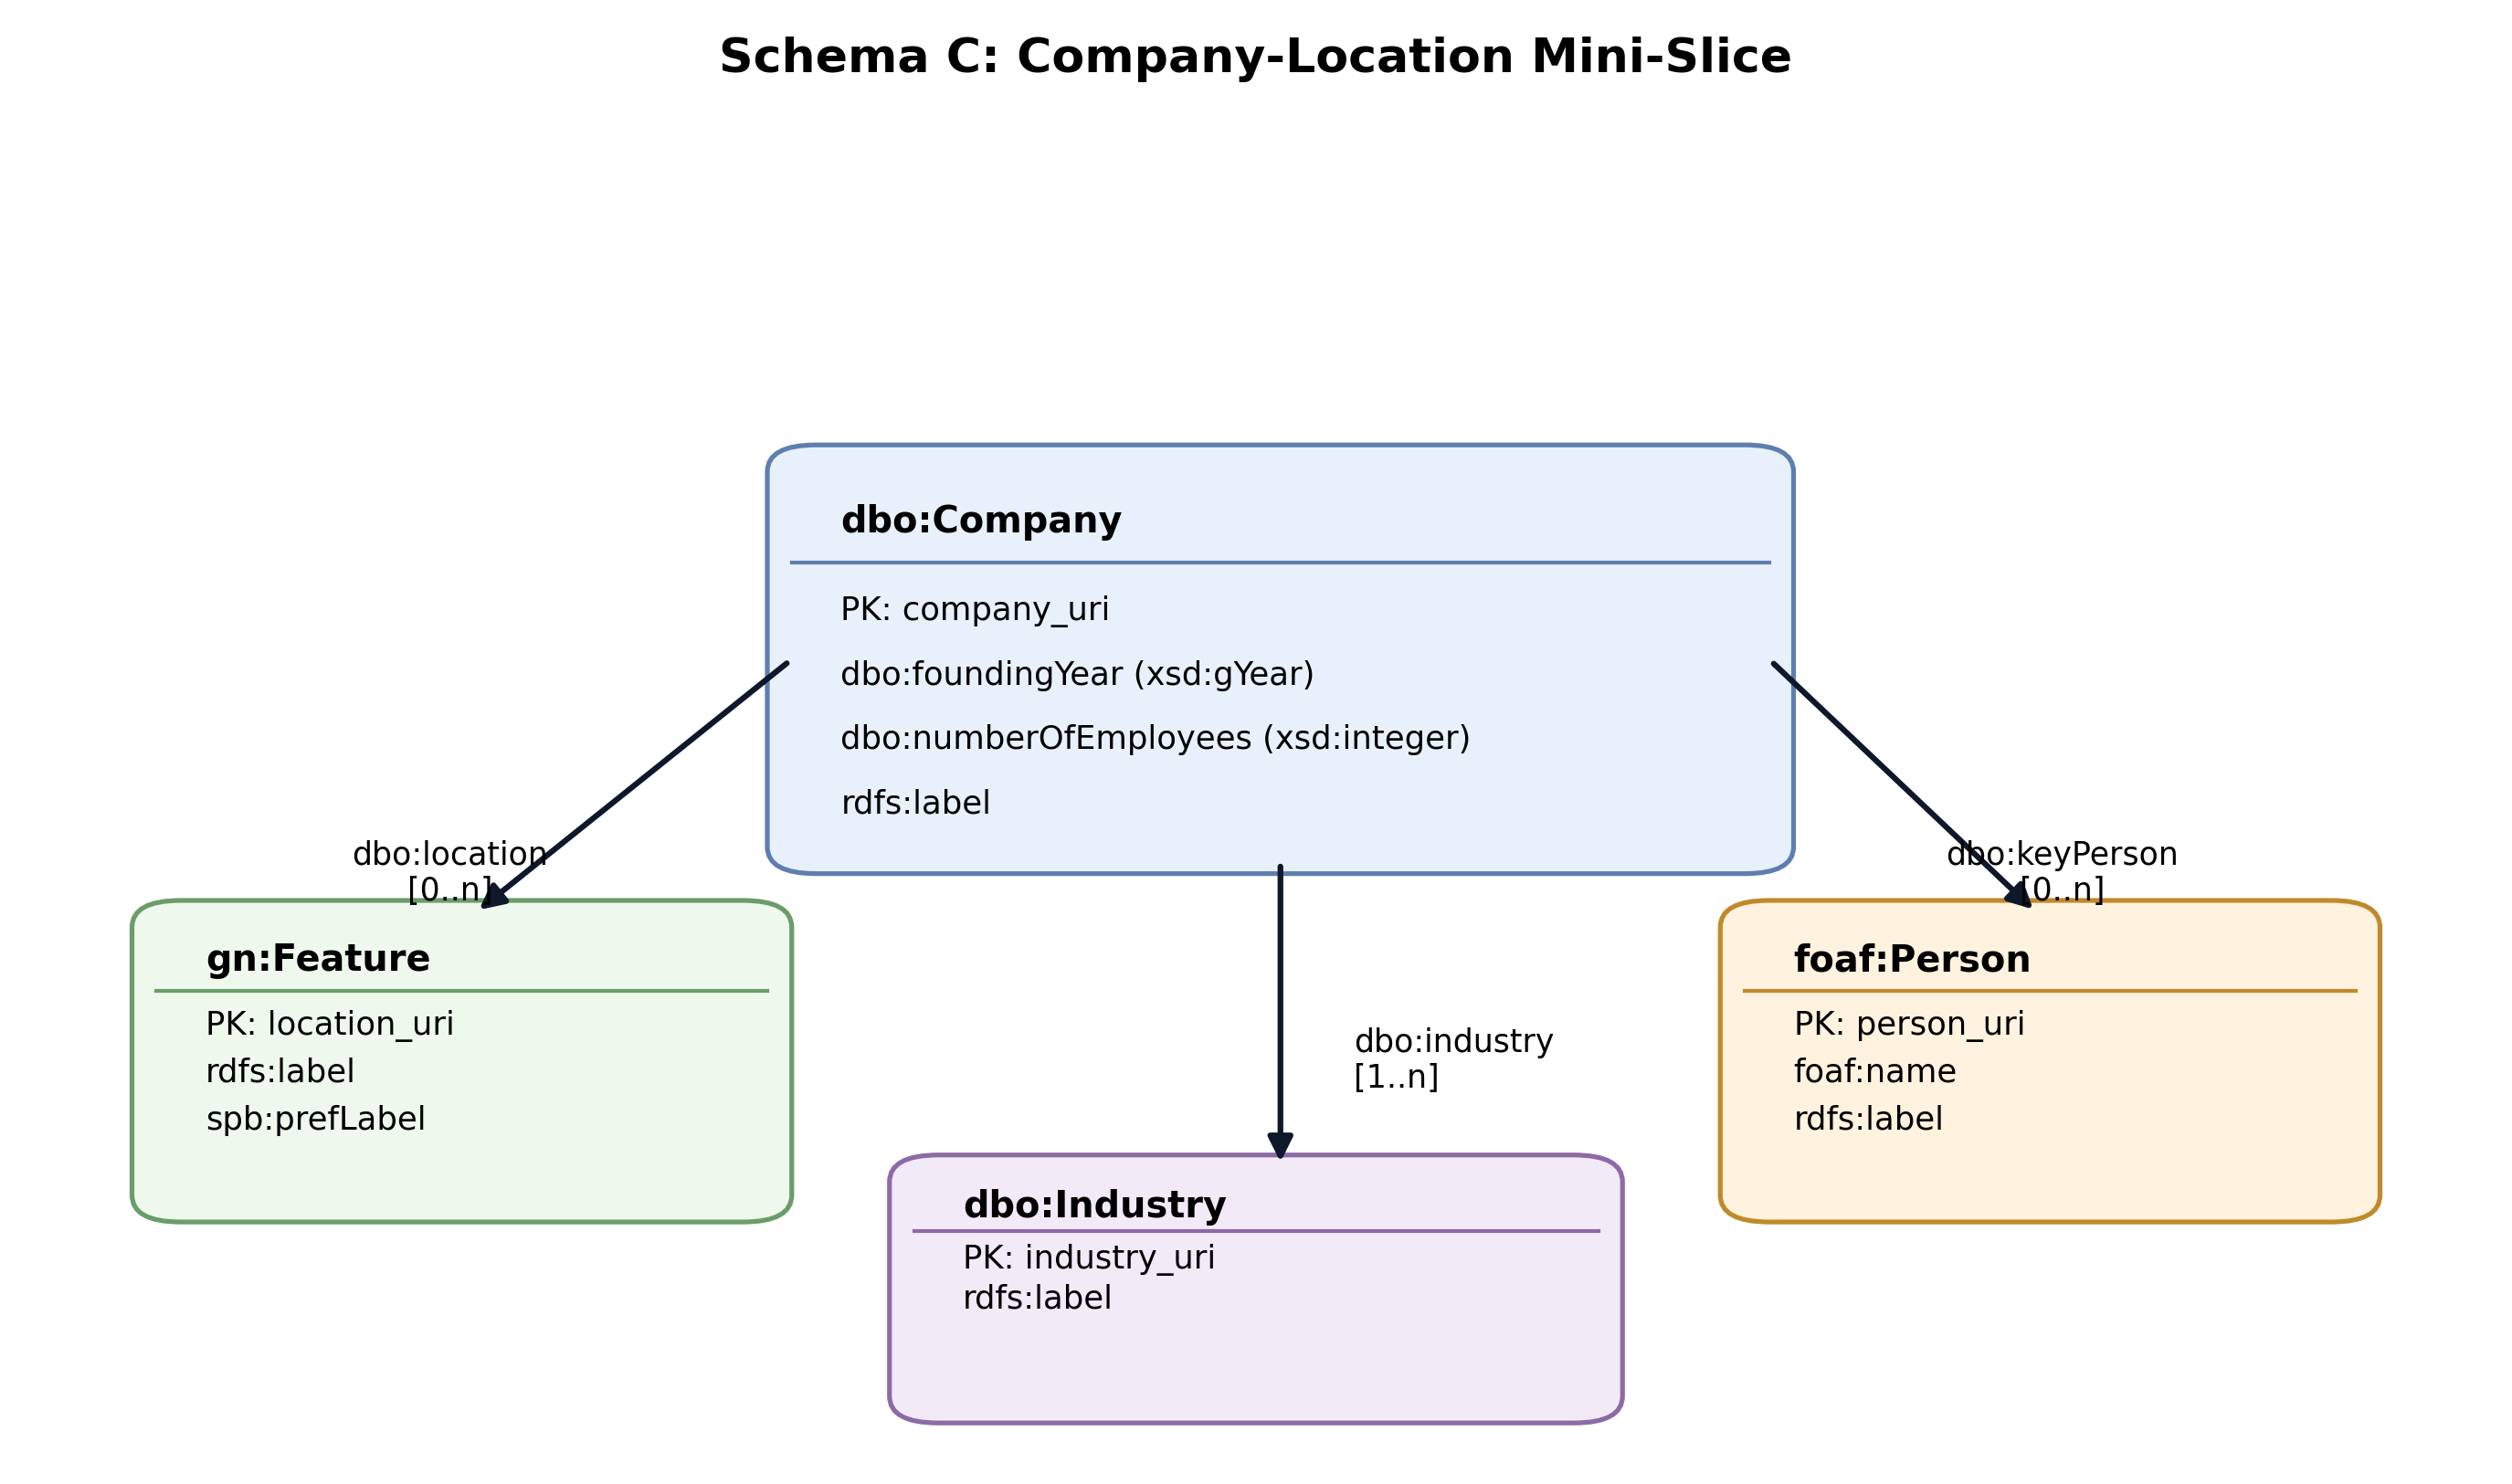
\includegraphics[width=0.95\linewidth]{figures/schema_ontology.png}
  \caption{Schema C mini-slice used in this study. \texttt{dbo:Company} connects to typed \texttt{gn:Feature} locations and \texttt{foaf:Person} key people; industry is represented as a labeled IRI-valued attribute and may not have an explicit type in the slice.}
  \label{fig:app_schema_ontology}
\end{figure}

\section{Example NL--SPARQL Pairs}
We include representative Phase-3 examples covering entity lookup, aggregation, boolean comparison, ranking, and conjunction. Prefix declarations are omitted for brevity; the artifact bundle contains full examples for all nine categories.

\noindent\textbf{Generic.} Q: Who is a key person at (Company: Volkswagen)?
\begin{SPARQL}
SELECT ?name
WHERE {
  VALUES ?company { <http://dbpedia.org/resource/Volkswagen> }
  ?company rdf:type dbo:Company .
  ?company dbo:keyPerson ?person .
  ?person rdf:type foaf:Person .
  ?person foaf:name ?name .
}
LIMIT 5
\end{SPARQL}

\noindent\textbf{Counting.} Q: How many companies are located in (Location: Menlo Park, California)?
\begin{SPARQL}
SELECT (COUNT(DISTINCT ?company) AS ?count)
WHERE {
  VALUES ?location { <http://dbpedia.org/resource/Menlo_Park,_California> }
  ?company a dbo:Company .
  ?company dbo:location ?location .
  ?location a gn:Feature .
}
\end{SPARQL}

\noindent\textbf{Comparative.} Q: Do (Company: Airbus) and (Company: FileMaker Inc.) have different numbers of employees?
\begin{SPARQL}
ASK {
  VALUES ?company1 { <http://dbpedia.org/resource/Airbus> }
  VALUES ?company2 { <http://dbpedia.org/resource/FileMaker_Inc.> }
  ?company1 a dbo:Company .
  ?company2 a dbo:Company .
  ?company1 dbo:numberOfEmployees ?n1 .
  ?company2 dbo:numberOfEmployees ?n2 .
  FILTER (xsd:integer(?n1) != xsd:integer(?n2))
}
\end{SPARQL}

\noindent\textbf{Ordinal.} Q: Which company was founded second earliest?
\begin{SPARQL}
SELECT ?company ?year
WHERE {
  ?company a dbo:Company .
  ?company dbo:foundingYear ?year .
}
ORDER BY ASC(xsd:integer(?year)) ?company
OFFSET 1
LIMIT 1
\end{SPARQL}

\noindent\textbf{Intersection.} Q: Which companies are located in (Location: California) and are in the (Industry: Software)?
\begin{SPARQL}
SELECT DISTINCT ?company
WHERE {
  ?company a dbo:Company .
  ?company dbo:location <http://dbpedia.org/resource/California> .
  ?company dbo:industry <http://dbpedia.org/resource/Software> .
}
LIMIT 5
\end{SPARQL}

\end{document}
